\documentclass{beamer}
\usepackage{tikz,amsmath,hyperref,graphicx,stackrel}
\usetikzlibrary{positioning,shadows,arrows,shapes,calc,dsp,chains}
\newcommand{\argmax}{\operatornamewithlimits{argmax}}
\newcommand{\argmin}{\operatornamewithlimits{argmin}}
\mode<presentation>{\usetheme{Frankfurt}}
\AtBeginSection[]
{
  \begin{frame}<beamer>
    \frametitle{Outline}
    \tableofcontents[currentsection,currentsubsection]
  \end{frame}
}
\title{Lecture 14: Cascaded LSI Systems}
\author{Mark Hasegawa-Johnson}
\date{ECE 401: Signal and Image Analysis, Fall 2021}  
\begin{document}

% Title
\begin{frame}
  \maketitle
\end{frame}

% Title
\begin{frame}
  \tableofcontents
\end{frame}

%%%%%%%%%%%%%%%%%%%%%%%%%%%%%%%%%%%%%%%%%%%%
\section[Review]{Review: Frequency Response and Fourier Series}
\setcounter{subsection}{1}

\begin{frame}
  \frametitle{Review: Convolution}
  \begin{itemize}
  \item A {\bf convolution} is exactly the same thing as a {\bf weighted local average}.
    We give it a special name, because we will use it very often.  It's defined as:
    \[
    y[n] = \sum_m g[m] f[n-m] = \sum_m g[n-m] f[m]
    \]
  \item 
    We use the symbol $\ast$ to mean ``convolution:''
    \[
    y[n]=g[n]\ast f[n] = \sum_m g[m] f[n-m] = \sum_m g[n-m] f[m]
    \]
  \end{itemize}
\end{frame}

\begin{frame}
  \frametitle{Frequency Response}
  \begin{itemize}
  \item {\bf Tones in $\rightarrow$ Tones out}
    \begin{align*}
      x[n]=e^{j\omega n} &\rightarrow y[n]=G(\omega)e^{j\omega n}\\
      x[n]=\cos\left(\omega n\right)
      &\rightarrow y[n]=|G(\omega)|\cos\left(\omega n+\angle G(\omega)\right)\\
      x[n]=A\cos\left(\omega n+\theta\right)
      &\rightarrow y[n]=A|G(\omega)|\cos\left(\omega n+\theta+\angle G(\omega)\right)
    \end{align*}
  \item where the {\bf Frequency Response} is given by
    \[
    G(\omega) = \sum_m g[m]e^{-j\omega m}
    \]
  \end{itemize}
\end{frame}

\begin{frame}
  \frametitle{Review: Spectrum}

  The {\bf spectrum} of $x(t)$ is the set of frequencies, and their
  associated phasors,
  \[
  \mbox{Spectrum}\left( x(t) \right) =
  \left\{ (f_{-N},a_{-N}), \ldots, (f_0,a_0), \ldots, (f_N,a_N) \right\}
  \]
  such that
  \[
  x(t) = \sum_{k=-N}^N a_ke^{j2\pi f_kt}
  \]
\end{frame}

\begin{frame}
  \frametitle{Review: Fourier Series}

  One reason the spectrum is useful is that {\bf\em any} periodic
  signal can be written as a sum of cosines.  Fourier's theorem says that
  any $x(t)$ that is periodic, i.e.,
  \[
  x(t+T_0) = x(t)
  \]
  can be written as
  \[
  x(t) = \sum_{k=-\infty}^\infty X_k e^{j2\pi k F_0 t}
  \]
  which is a special case of the spectrum for periodic signals:
  $f_k=kF_0$, and $a_k=X_k$, and
  \[
  F_0 = \frac{1}{T_0}
  \]
\end{frame}

\begin{frame}
  \frametitle{Review: Discrete-Time Fourier Series}

  A signal that's periodic in discrete time also has a Fourier series.
  If the signal is periodic with a period of $N_0=T_0F_s$ samples,
  then its Fourier series is
  \[
  x[n] = \sum_{k=0}^{N_0-1} X_k e^{j2\pi kn/N_0} =\sum_{k=-N_0/2}^{(N_0-1)/2} X_k e^{j2\pi kn/N_0}
  \]
  and the Fourier analysis formula is
  \[
  X_k = \frac{1}{N_0}\sum_{n=0}^{N_0-1} x[n]e^{-j2\pi kn/N_0}  
  \]
\end{frame}

\begin{frame}
  \frametitle{Example: Spectrum of a Square Wave}

  For example, here's an even-symmetric ($x[n]=x[-n]$), zero-DC
  ($\sum_n x[n]=0$), unit-amplitude ($\max_n |x[n]|=1$) square wave,
  with a period of 11 samples:
  \centerline{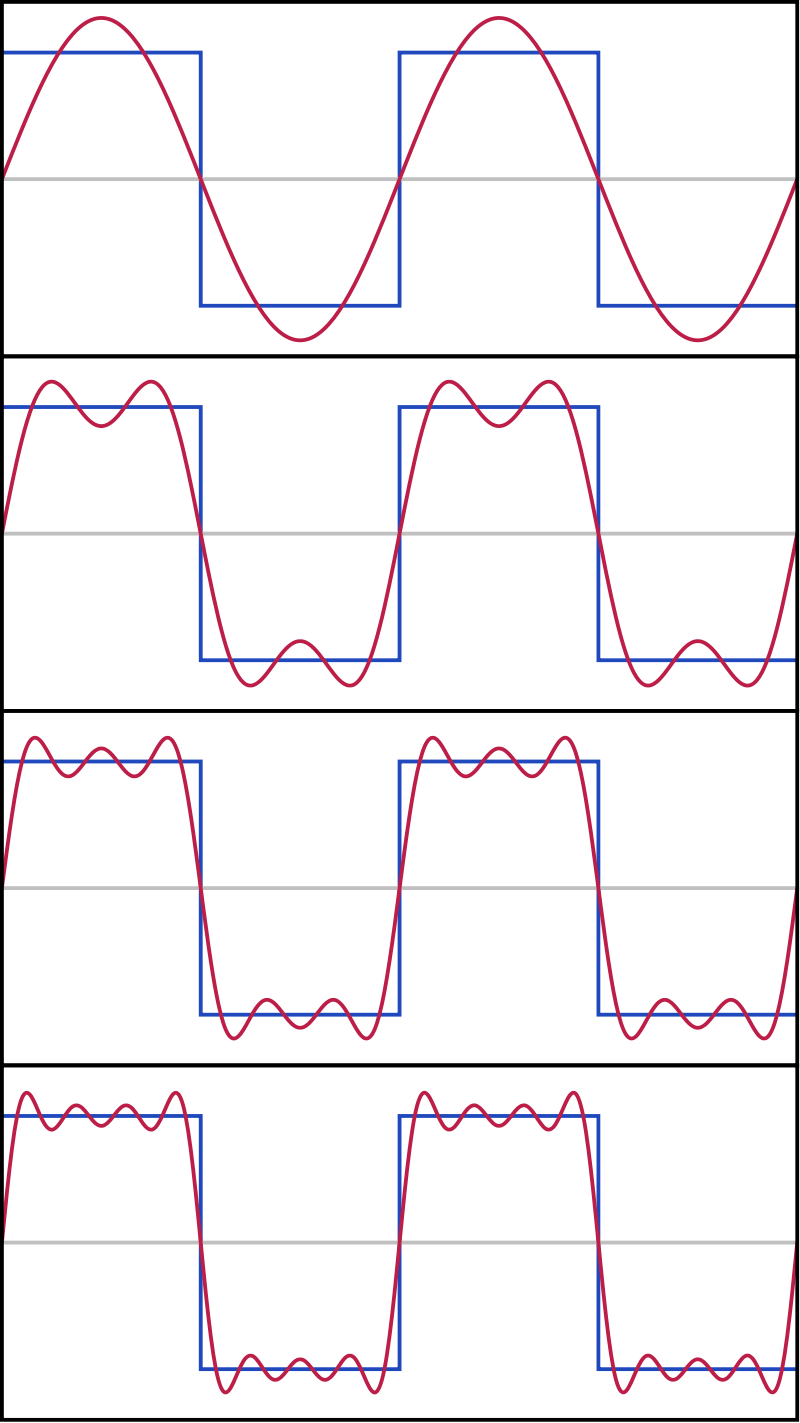
\includegraphics[height=2.5in]{exp/squarewave.png}}
\end{frame}

\begin{frame}
  \frametitle{Spectrum of a Square Wave}

  \centerline{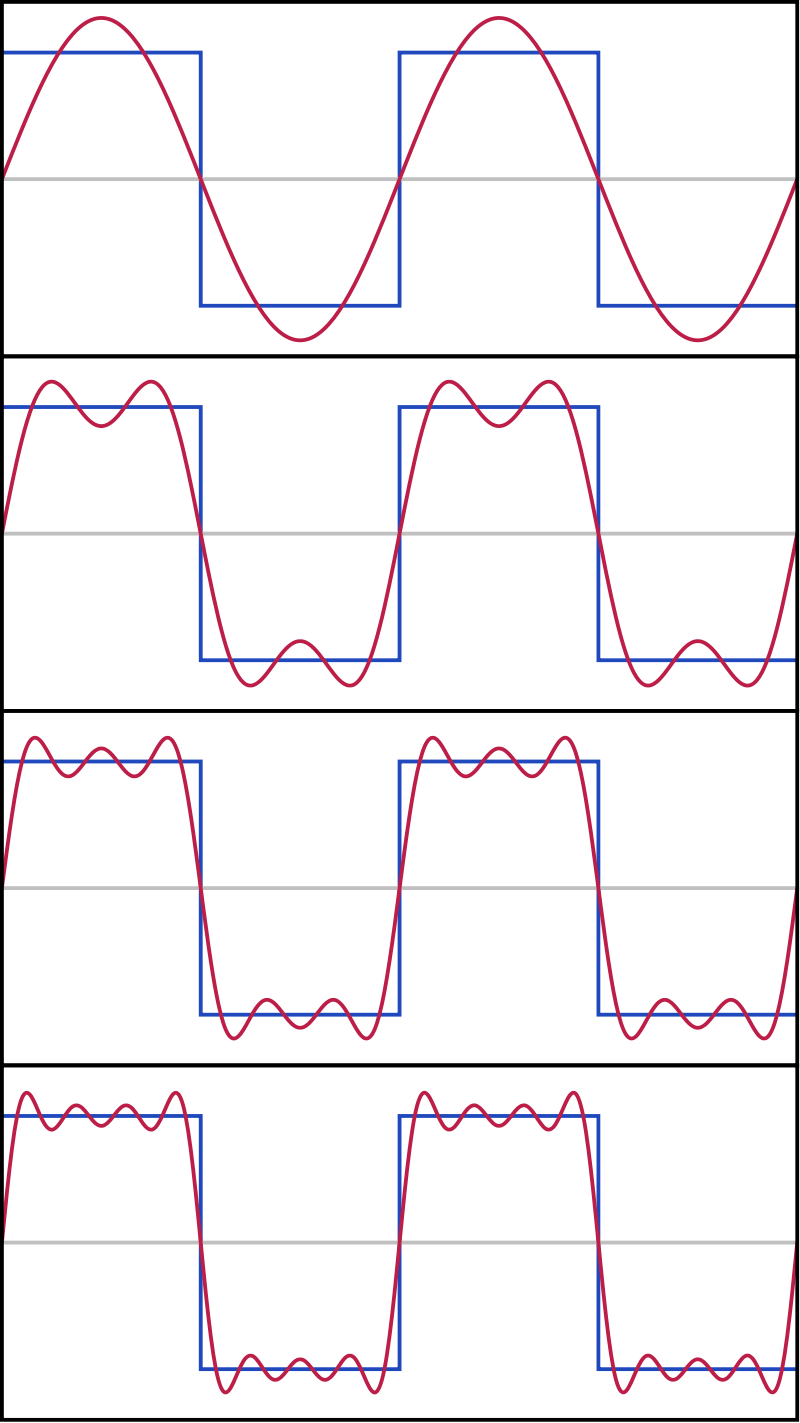
\includegraphics[height=1in]{exp/squarewave.png}}
  The Fourier series coefficients of this square wave are
  \[
  X_k = \begin{cases}
    \frac{2\pi}{k}(-1)^{\frac{|k|-1}{2}} & k~\mbox{odd},~-5\le k\le 5\\
    0 & k~\mbox{even},~-5\le k\le 5
  \end{cases}
  \]
\end{frame}

\begin{frame}
  \frametitle{More about the phase spectrum}
  \centerline{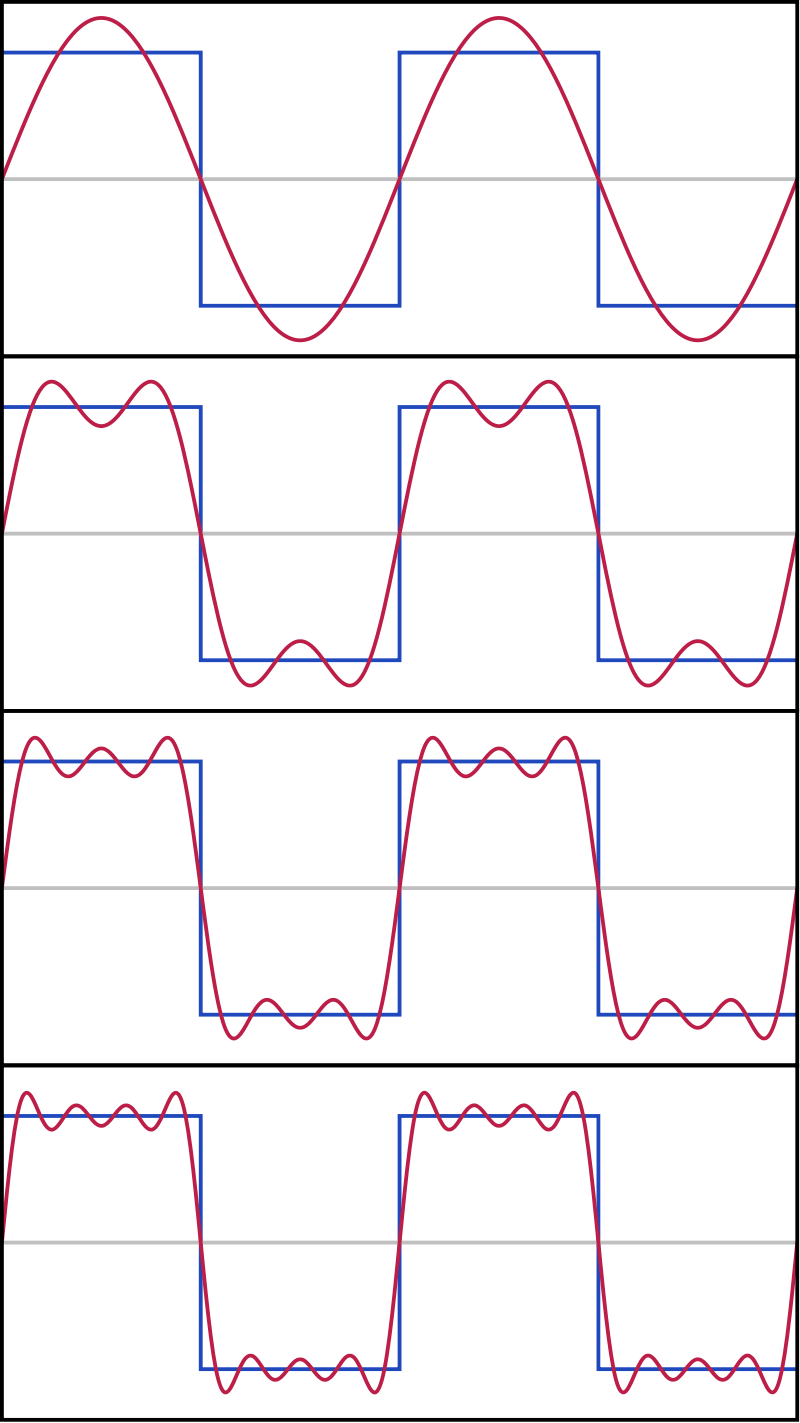
\includegraphics[height=1.5in]{exp/squarewave.png}}
  Notice that, for the phase spectrum of a square wave, the phase
  spectrum is either $\angle X[k]=0$ or $\angle X[k]=\pi$.  That means that the
  spectrum is real-valued, with no complex part:
  \begin{itemize}
  \item {\bf Positive real:} $X[k]=|X[k]|$
  \item {\bf Negative real:} $X[k]=-|X[k]| = |X[k]|e^{j\pi}$
  \end{itemize}
\end{frame}

\begin{frame}
  \frametitle{More about the phase spectrum}
  
  Having discovered that the square wave has a real-valued $X[k]$, we could
  just plot $X[k]$ itself, instead of plotting its magnitude and phase:
  \centerline{\includegraphics[height=2.5in]{exp/squarewave_real.png}}
\end{frame}


%%%%%%%%%%%%%%%%%%%%%%%%%%%%%%%%%%%%%%%%%%%%
\section[Periodic Signals]{Response of a Filter when the  Input is Periodic}
\setcounter{subsection}{1}

\begin{frame}
  \frametitle{Response of a Filter when the Input is Periodic}

  Now we're ready to ask this question:
  \begin{block}{}
    What is the output of a filter when the  input, $x[n]$, is periodic with
    period $N_0$?
  \end{block}
\end{frame}

\begin{frame}
  \frametitle{Response of a Filter when the Input is Periodic}

  \begin{enumerate}
  \item {\bf Fourier Series:}
    If the input is periodic, then we can write  it as
    \[
    x[n] =\sum_{k=-N_0/2}^{(N_0-1)/2} X_k e^{j2\pi kn/N_0}
    \]
  \item {\bf Frequency Response:}
    If the input is $e^{j\omega n}$, then the output is
    \[
    y[n] = H(\omega)e^{j\omega n}
    \]
  \item {\bf Linearity (of convolution, and of frequency response):}
    If the input is $x_1[n]+x_2[n]$, then the output is
    \[
    y[n] = y_1[n]+y_2[n]
    \]
  \end{enumerate}
\end{frame}

\begin{frame}
  \frametitle{Response of a Filter when the Input is Periodic}

  Putting all those things together, if the input is
  \[
  x[n] =\sum_{k=-N_0/2}^{(N_0-1)/2} X_k e^{j2\pi kn/N_0}
  \]
  \ldots then the output is
  \[
  y[n] = \sum_{k=-N_0/2}^{(N_0-1)/2} X_k H(k\omega_0) e^{j2\pi kn/N_0}
  \]
  \ldots where $\omega_0=\frac{2\pi}{N_0}$ is the fundamental frequency.
\end{frame}


%%%%%%%%%%%%%%%%%%%%%%%%%%%%%%%%%%%%%%%%%%%%
\section[Pure Delay]{A Pure-Delay ``Filter''}
\setcounter{subsection}{1}

\begin{frame}
  \frametitle{A Pure-Delay ``Filter''}

  One thing we can do to a signal is to just delay it, by $n_0$ samples:
  \[
  y[n] = x[n-n_0]
  \]
  Even this very simple operation can be written as a convolution:
  \[
  y[n]=g[n]\ast x[n]
  \]
  where the ``filter,'' $g[n]$, is just
  \[
  g[n]=\delta[n-n_0] = \begin{cases}
  1 & n=n_0\\
  0 & \mbox{otherwise}
  \end{cases}
  \]
\end{frame}

\begin{frame}
  \frametitle{Frequency Response of A Pure-Delay ``Filter''}

  \[
  g[n]=\begin{cases}
  1 & n=n_0\\
  0 & \mbox{otherwise}
  \end{cases}
  \]
  The frequency response is
  \[
  G(\omega)=\sum_m g[m]e^{-j\omega m} = e^{-j\omega n_0}
  \]
  
\end{frame}

\begin{frame}
  \frametitle{Impulse Response of A Pure-Delay ``Filter''}
  Here is the impulse response of a pure-delay ``filter'' (and the magnitude and
  phase responses, which we'll talk about next).
\centerline{\includegraphics[height=2.5in]{exp/puredelay.png}}
\end{frame}

\begin{frame}
  \frametitle{Magnitude and Phase Response of A Pure-Delay ``Filter''}

  \[
  G(\omega)=\sum_m g[m]e^{-j\omega m} = e^{-j\omega n_0}
  \]
  Notice that the magnitude and phase response of this filter are
  \begin{align*}
    |G(\omega)| &= 1\\
    \angle G(\omega) &= -\omega n_0
  \end{align*}
  So, for example, if have an input of $x[n]=\cos(\omega n)$, the
  output would be
  \[
  y[n]=|G(\omega)|\cos\left(\omega n+\angle G(\omega)\right)
  = \cos\left(\omega n-\omega n_0\right)
  \]
\end{frame}


%%%%%%%%%%%%%%%%%%%%%%%%%%%%%%%%%%%%%%%%%%%%
\section[Example]{Example: Delaying a Square Wave}
\setcounter{subsection}{1}

\begin{frame}
  \frametitle{Magnitude and Phase Response of A Pure-Delay ``Filter''}
  Here are the magnitude and phase response of the pure delay filter.
\centerline{\includegraphics[height=2.5in]{exp/puredelay.png}}
\end{frame}

\begin{frame}
  \frametitle{Spectrum of a Square Wave}

  \centerline{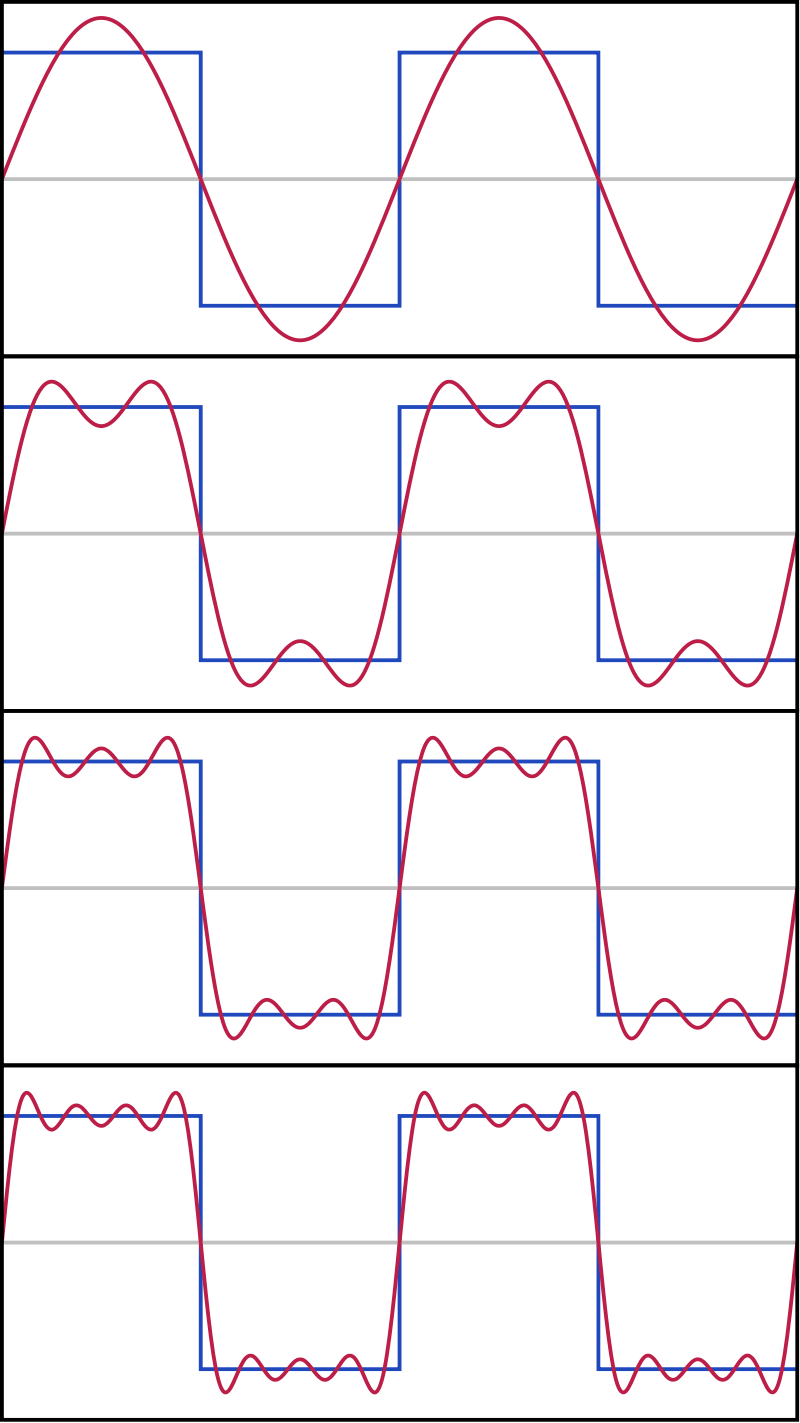
\includegraphics[height=1in]{exp/squarewave.png}}

  Here are the Fourier series coefficients of a period-11,
  even-symmetric, unit-amplitude, zero-mean square wave:
  \[
  X_k = \begin{cases}
    \frac{2\pi}{k}(-1)^{\frac{|k|-1}{2}} & k~\mbox{odd},~-5\le k\le 5\\
    0 & k~\mbox{even},~-5\le k\le 5
  \end{cases}
  \]
\end{frame}

\begin{frame}
  \frametitle{Response of a Filter when the Input is Periodic}

  And here's what happens when we pass a periodic signal through a filter $g[n]$:
  \[
  x[n] =\sum_{k=-N_0/2}^{(N_0-1)/2} X_k e^{j2\pi kn/N_0}
  \]
  \[
  y[n] = \sum_{k=-N_0/2}^{(N_0-1)/2} X_k G(k\omega_0) e^{j2\pi kn/N_0}
  \]
  \ldots where $\omega_0=\frac{2\pi}{N_0}$ is the fundamental frequency.
\end{frame}

\begin{frame}
  \frametitle{Spectrum: Delayed Square Wave} And here's the result.
  This is the square wave, after being delayed by the pure-delay
  filter:
  \centerline{\includegraphics[height=2.5in]{exp/delayedsquarewave.png}}
  You can see that magnitude's unchanged, but phase is changed.
\end{frame}

\begin{frame}
  \frametitle{Spectrum of a Delayed Square Wave}

  \centerline{\includegraphics[height=1in]{exp/delayedsquarewave.png}}
  The Fourier series coefficients of a square wave, delayed by $n_0$
  samples, are
  \[
  Y_k = \begin{cases}
    \frac{2\pi}{k}(-1)^{\frac{|k|-1}{2}}e^{-jk\omega_0 n_0} & k~\mbox{odd},~-5\le k\le 5\\
    0 & k~\mbox{even},~-5\le k\le 5
  \end{cases}
  \]
  where $k\omega_0=\frac{2\pi k}{N_0}$.
\end{frame}


%%%%%%%%%%%%%%%%%%%%%%%%%%%%%%%%%%%%%%%%%%%%
\section[Cascades]{Cascaded LSI Systems}
\setcounter{subsection}{1}

\begin{frame}
  \frametitle{Cascaded LSI Systems}

  What happens if we pass the input through two LSI systems, in cascade?
  \begin{center}
    \begin{tikzpicture}
      \node[dspnodeopen,dsp/label=right] (y) at (7.5,0) {$y[n]$};
      \node[dspsquare] (h) at (5,0) {${\mathcal H}$} edge[dspconn](y);
      \node[dspsquare] (g) at (2.5,0) {${\mathcal G}$} edge[dspconn](h);
      \node[dspnodeopen,dsp/label=left] (x) at (0,0) {$x[n]$} edge[dspconn](g);
    \end{tikzpicture}
  \end{center}
\end{frame}
  
\begin{frame}
  \frametitle{Cascaded filters}

  Suppose I pass the signal through filter $g[n]$, then pass it through
  another filter, $h[n]$:
  \[
  y[n]=h[n]\ast \left(g[n]\ast x[n]\right),
  \]
  we get a signal $y[n]$ whose spectrum is:
  \[
  Y[k]=H(k\omega_0) G(k\omega_0) X[k]
  \]
\end{frame}


\begin{frame}
  \frametitle{Convolution  is Commutative}

  Notice that
  \[
  Y[k] = H(k\omega_0) G(k\omega_0) X[k]=G(k\omega_0)H(k\omega_0) X[k]
  \]
  and therefore:
  \[
  y[n]=h[n]\ast \left(g[n]\ast x[n]\right)=g[n]\ast \left(h[n]\ast x[n]\right)
  \]
\end{frame}

\begin{frame}
  \frametitle{Convolution  is Commutative}

  Since convolution is commutative, these two circuits compute exactly the same output:
  \begin{center}
    \begin{tikzpicture}
      \node[dspnodeopen,dsp/label=right] (y) at (7.5,0) {$y[n]$};
      \node[dspsquare] (h) at (5,0) {${\mathcal H}$} edge[dspconn](y);
      \node[dspsquare] (g) at (2.5,0) {${\mathcal G}$} edge[dspconn](h);
      \node[dspnodeopen,dsp/label=left] (x) at (0,0) {$x[n]$} edge[dspconn](g);
    \end{tikzpicture}
  \end{center}
  \begin{center}
    \begin{tikzpicture}
      \node[dspnodeopen,dsp/label=right] (y) at (7.5,0) {$y[n]$};
      \node[dspsquare] (g) at (5,0) {${\mathcal G}$} edge[dspconn](y);
      \node[dspsquare] (h) at (2.5,0) {${\mathcal H}$} edge[dspconn](g);
      \node[dspnodeopen,dsp/label=left] (x) at (0,0) {$x[n]$} edge[dspconn](h);
    \end{tikzpicture}
  \end{center}
\end{frame}

  
\begin{frame}
  \frametitle{Example: Differenced Square Wave}

  Suppose we define $x[n]$ to be an 11-sample square wave,
  $g[n]$ to be a delay, and $h[n]$ to be a first difference:
  \[
  x[n] = \begin{cases}
    1 & -2\le n\le 2\\
    -\frac{1}{2} & n=\pm 3\\
    -1 & 4\le n\le 7
  \end{cases}
  \]
  \[
  x[n] \stackrel{\mathcal G}{\longrightarrow} z[n] = x[n-5]
  \]
  \[
  z[n] \stackrel{\mathcal H}{\longrightarrow} y[n] = z[n]-z[n-1]
  \]
\end{frame}

\begin{frame}
  \frametitle{Delayed Square Wave}
  
  \begin{center}
    \begin{tikzpicture}
      \node[dspnodeopen,dsp/label=right] (y) at (5,0) {$y[n]$};
      \node[dspsquare] (g) at (2.5,0) {${\mathcal G}$} edge[dspconn](y);
      \node[dspnodeopen,dsp/label=left] (x) at (0,0) {$x[n]$} edge[dspconn](g);
    \end{tikzpicture}
  \end{center}
  Here's what we get if we just {\bf delay} the square wave:
  \centerline{\includegraphics[height=2in]{exp/delayedsquarewave.png}}
\end{frame}

\begin{frame}
  \frametitle{Differenced Square Wave}
  
  \begin{center}
    \begin{tikzpicture}
      \node[dspnodeopen,dsp/label=right] (y) at (5,0) {$y[n]$};
      \node[dspsquare] (g) at (2.5,0) {${\mathcal H}$} edge[dspconn](y);
      \node[dspnodeopen,dsp/label=left] (x) at (0,0) {$x[n]$} edge[dspconn](g);
    \end{tikzpicture}
  \end{center}
  Here's what we get if we just {\bf difference} the square wave:
  \centerline{\includegraphics[height=2in]{exp/differenced_squarewave.png}}
\end{frame}

\begin{frame}
  \frametitle{Example: Differenced Delayed Square Wave}

  \begin{center}
    \begin{tikzpicture}
      \node[dspnodeopen,dsp/label=right] (y) at (7.5,0) {$y[n]$};
      \node[dspsquare] (h) at (5,0) {${\mathcal H}$} edge[dspconn](y);
      \node[dspsquare] (g) at (2.5,0) {${\mathcal G}$} edge[dspconn](h);
      \node[dspnodeopen,dsp/label=left] (x) at (0,0) {$x[n]$} edge[dspconn](g);
    \end{tikzpicture}
  \end{center}
  Here's what we get if we {\bf delay} and then {\bf difference} the square wave:
  \centerline{\includegraphics[height=2.5in]{exp/differenced_delayed_squarewave.png}}
\end{frame}

\begin{frame}
  \frametitle{Example: Delayed Differenced Square Wave}

  \begin{center}
    \begin{tikzpicture}
      \node[dspnodeopen,dsp/label=right] (y) at (7.5,0) {$y[n]$};
      \node[dspsquare] (h) at (5,0) {${\mathcal G}$} edge[dspconn](y);
      \node[dspsquare] (g) at (2.5,0) {${\mathcal H}$} edge[dspconn](h);
      \node[dspnodeopen,dsp/label=left] (x) at (0,0) {$x[n]$} edge[dspconn](g);
    \end{tikzpicture}
  \end{center}
  Here's what we get if we {\bf difference} and then {\bf delay} the square wave
  (hint: it's exactly the same as the previous slide!!)  
  \centerline{\includegraphics[height=2.5in]{exp/delayed_differenced_squarewave.png}}
\end{frame}

\begin{frame}
  \frametitle{Magnitude and Phase of Cascaded Frequency Responses}

  In general, when you cascade two LSI systems, the magnitudes multiply:
  \[
  |Y_k|=|H(\omega)||G(\omega)||X_k|,
  \]
  but the phases add:
  \[
  \angle Y_k = \angle H(\omega)+\angle G(\omega)+\angle X_k
  \]
  That's because:
  \[
  H(\omega)G(\omega)=|H(\omega)|e^{j\angle H(\omega)}|G(\omega)|e^{j\angle G(\omega)}
  =|H(\omega)||G(\omega)| e^{j\left(\angle H(\omega)+\angle G(\omega)\right)}
  \]
\end{frame}


%%%%%%%%%%%%%%%%%%%%%%%%%%%%%%%%%%%%%%%%%%%%
\section[Sum]{The Running-Sum Filter (Local Averaging)}
\setcounter{subsection}{1}

\begin{frame}
  \frametitle{Local Average Filters}

  Let's go back to the local averaging filter. I want to define two 
  different types of local average: centered, and delayed.
  \begin{itemize}
  \item {\bf Centered local average:} This one averages
    $\left(\frac{L-1}{2}\right)$ future samples,
    $\left(\frac{L-1}{2}\right)$ past samples, and $x[n]$:
    \[
    y_c[n] = \frac{1}{L}\sum_{m=-\left(\frac{L-1}{2}\right)}^{\left(\frac{L-1}{2}\right)} x[n-m]
    \]
  \item {\bf Delayed local average:} This one averages $x[n]$ and $L-1$ of its
    past samples:
    \[
    y_d[n] = \frac{1}{L}\sum_{m=0}^{L-1} x[n-m]
    \]
  \end{itemize}
  Notice that $y_d[n] = y_c\left[n-\left(\frac{L-1}{2}\right)\right]$.
\end{frame}

\begin{frame}
  \frametitle{Local Average Filters}

  We can write both of these as filters:
  \begin{itemize}
  \item {\bf Centered local average:}
    \begin{align*}
      y_c[n] &= f_c[n]\ast x[n]\\
      f_c[n] &= \begin{cases} \frac{1}{L}& -\left(\frac{L-1}{2}\right)\le n\le\left(\frac{L-1}{2}\right)\\
        0&\mbox{otherwise}\end{cases}
    \end{align*}
  \item {\bf Delayed local average:}
    \begin{align*}
      y_d[n] &= f_d[n]\ast x[n]\\
      f_d[n] &= \begin{cases} \frac{1}{L}& 0\le n\le L-1\\
        0&\mbox{otherwise}\end{cases}
    \end{align*}
  \end{itemize}
\end{frame}

\begin{frame}
  \frametitle{Local Average Filters}
  \centerline{\includegraphics[height=2.5in]{exp/localaveragefilters.png}}
  Notice that $f_d[n]=f_c\left[n-\left(\frac{L-1}{2}\right)\right]$.
\end{frame}  

\begin{frame}
  \frametitle{The relationship between centered local average and delayed local average}

  Suppose we define our pure delay filter,
  \[
  g[n]=\delta\left[n-\frac{L-1}{2}\right] = \begin{cases}
  1 & n=\frac{L-1}{2}\\
  0 & \mbox{otherwise}
  \end{cases}
  \]
  Using $g[n]$, here are  lots of different ways we can write the relationship
  between $y_d[n]$, $y_c[n]$, and $x[n]$:
  \begin{align*}
    y_d[n] &= f_d[n]\ast x[n]\\
    y_c[n] &= f_c[n]\ast x[n]\\
    y_d[n] &= g[n]\ast y_c[n] = g[n]\ast f_c[n]\ast x[n]\\
    f_d[n] &= g[n]\ast f_c[n]
  \end{align*}
\end{frame}
  
\begin{frame}
  \frametitle{The relationship between centered local average and delayed local average}

  Remember the frequency response of a pure delay filter:
  \[
  G(\omega)  = e^{-j\omega\left(\frac{L-1}{2}\right)}
  \]
  We have not yet figured out what $F_c(\omega)$ and $F_d(\omega)$
  are.  But whatever they are, we know that
  \[
  f_d[n] = g[n]\ast f_c[n]
  \]
  and therefore
  \[
  F_d(\omega) = e^{-j\omega\left(\frac{L-1}{2}\right)} F_c(\omega)
  \]
\end{frame}
  
\begin{frame}
  \frametitle{The frequency response of a local average filter}

  Let's find the frequency response of
  \[
  f_d[n] = \begin{cases} \frac{1}{L}& 0\le m\le L-1\\
    0&\mbox{otherwise}\end{cases}
  \]
  The formula is
  \[
  F_d(\omega) = \sum_m f[m]e^{-j\omega m},
  \]
  so,
  \[
  F_d(\omega) = \sum_{m=0}^{L-1} \frac{1}{L}e^{-j\omega m}
  \]
\end{frame}
  
\begin{frame}
  \frametitle{The frequency response of a local average filter}

  \[
  F_d(\omega) = \sum_{m=0}^{L-1} \frac{1}{L}e^{-j\omega m}
  \]
  This is just a standard geometric series,
  \[
  \sum_{m=0}^{L-1} a^m = \frac{1-a^L}{1-a},
  \]
  so:
  \[
  F_d(\omega) = \frac{1}{L}\left(\frac{1-e^{-j\omega L}}{1-e^{-j\omega}}\right)
  \]
\end{frame}
  
\begin{frame}
  \frametitle{The frequency response of a local average filter}

  We now have an extremely  useful transform pair:
  \[
  f_d[n] = \begin{cases} \frac{1}{L}& 0\le m\le L-1\\
    0&\mbox{otherwise}\end{cases}~~~\leftrightarrow~~~
  F_d(\omega) = \frac{1}{L}\left(\frac{1-e^{-j\omega L}}{1-e^{-j\omega}}\right)
  \]
  Let's attempt to convert that into polar form, so we can find
  magnitude and phase response. Notice that both the numerator and the
  denominator are subtractions of complex numbers, so we might be able
  to use $2j\sin(x)=e^{jx}-e^{-jx}$ for some $x$.  Let's try:
  \begin{align*}
    \frac{1}{L}\left(\frac{1-e^{-j\omega L}}{1-e^{-j\omega}}\right)
    &= \frac{1}{L}\frac{e^{-j\omega L/2}}{e^{-j\omega/2}}
    \left(\frac{e^{j\omega L/2}-e^{-j\omega L/2}}{e^{j\omega/2}-e^{-j\omega/2}}\right)\\
    &= e^{-j\omega\left(\frac{L-1}{2}\right)}\frac{1}{L}
    \left(\frac{2j\sin(\omega L/2)}{2j\sin(\omega/2)}\right)\\
    &= e^{-j\omega\left(\frac{L-1}{2}\right)}\frac{1}{L}
    \left(\frac{\sin(\omega L/2)}{\sin(\omega/2)}\right)
  \end{align*}
\end{frame}
  
\begin{frame}
  \frametitle{The frequency response of a local average filter}

  Now we have $F_d(\omega)$ in almost magnitude-phase form:
  \[
  f_d[n] = \begin{cases} \frac{1}{L}& 0\le m\le L-1\\
    0&\mbox{otherwise}\end{cases}~~~\leftrightarrow~~~
  F_d(\omega)=\left(\frac{\sin(\omega L/2)}{L\sin(\omega/2)}\right)e^{-j\omega\left(\frac{L-1}{2}\right)}
  \]
  By the way, remember we discovered that
  \[
  f_d[n]=g[n]\ast f_c[n]~~~\leftrightarrow~~~F_d(\omega)=e^{-j\omega\left(\frac{L-1}{2}\right)}F_c(\omega)
  \]
  Notice anything?
\end{frame}

\begin{frame}
  \frametitle{Dirichlet form}

  The textbook calls this function the ``Dirichlet form:''
  \[
  D_L(\omega) = \frac{\sin(\omega L/2)}{\sin(\omega/2)}
  \]
  That is, exactly, the frequency response of a centered local sum filter:
  \[
  d_L[n] = \begin{cases}
    1 & -\left(\frac{L-1}{2}\right)\le n\le \left(\frac{L-1}{2}\right)\\
    0 & \mbox{otherwise}
  \end{cases}
  \]
\end{frame}

\begin{frame}
  \frametitle{Dirichlet form}

  Here's what it looks like:
  \centerline{\includegraphics[height=2.5in]{exp/dirichletform.png}}
\end{frame}
  
\begin{frame}
  \frametitle{Dirichlet form}

  Since every local averaging filter is based on Dirichlet form, it's
  worth spending some time to understand it better.
  \[
  D_L(\omega) = \frac{\sin(\omega L/2)}{\sin(\omega/2)}
  \]
  \begin{itemize}
  \item It's equal to zero every time $\omega L/2$ is a multiple of $\pi$.  So
    \[
    D_L\left(\frac{2\pi k}{L}\right)  = 0~~\mbox{for all integers}~k~\mbox{except}~k=0
    \]
  \item At $\omega=0$, the value of $\frac{\sin(\omega
    L/2)}{\sin(\omega/2)}$ is undefined, but it's posssible to prove
    that $\lim_{\omega\rightarrow 0}D_L(\omega)=L$.  To make life
    easy, we'll just define it that way:
    \[
    \mbox{DEFINE:}~~D_L(0)=L
    \]
  \end{itemize}
\end{frame}

\begin{frame}
  \frametitle{Dirichlet form}

  Here's what it looks like:
  \centerline{\includegraphics[height=2.5in]{exp/dirichletform.png}}
\end{frame}
  
\begin{frame}
  \frametitle{Local averaging filter}

  Here's what the centered local averaging filter looks like.  Notice that
  it's just $1/L$ times the Dirichlet form:
  \centerline{\includegraphics[height=2.5in]{exp/centeredaveragingfilter.png}}
\end{frame}
  

%%%%%%%%%%%%%%%%%%%%%%%%%%%%%%%%%%%%%%%%%%%%
\section[Summary]{Summary}
\setcounter{subsection}{1}

\begin{frame}
  \frametitle{Summary: Behavior of Systems in General}
  \begin{itemize}
  \item {\bf Periodic inputs:}
    If the input of an LSI system is periodic,
    \[
    x[n] =\sum_{k=-N_0/2}^{(N_0-1)/2} X_k e^{j2\pi kn/N_0}
    \]
    \ldots then the output is
    \[
    y[n] = \sum_{k=-N_0/2}^{(N_0-1)/2} X_k H(k\omega_0) e^{j2\pi kn/N_0}
    \]
  \item {\bf Cascaded LTI Systems} convolve their impulse responses, equivalently, they
    multiply their frequency responses:
    \[
    y[n]=h[n]\ast g[n]\ast x[n],~~~Y_k=H(k\omega_0)G(k\omega_0)X_k
    \]
  \end{itemize}
\end{frame}

\begin{frame}
  \frametitle{Summary: Types of LSI Systems}
  \begin{itemize}
  \item The {\bf Pure Delay Filter} has $|G(\omega)|=1$, $\angle G(\omega)=-\omega n_0$:
    \[
    g[m]=\delta[n-n_0]~~~\leftrightarrow~~~G(\omega) = e^{-j\omega n_0}
    \]
  \item The {\bf Centered Local Averaging Filter} is $1/L$ times
    the Dirichlet form:
    \[
    f_c[n] = \begin{cases}
      \frac{1}{L} & -\left(\frac{L-1}{2}\right)\le n\le \left(\frac{L-1}{2}\right)\\
      0 & \mbox{otherwise}
    \end{cases}~~~\leftrightarrow~~~
    F_c(\omega)=\frac{\sin(\omega L/2)}{L\sin(\omega/2)}
    \]
  \item The {\bf Delayed Local Averaging Filter} is $f_c[n]$, delayed by half of its length:
    \[
    f_d[n] = \begin{cases}
      \frac{1}{L} & 0\le n\le L-1\\
      0 & \mbox{otherwise}
    \end{cases}~~~\leftrightarrow~~~
    F_d(\omega)=\frac{\sin(\omega L/2)}{L\sin(\omega/2)}e^{-j\omega\left(\frac{L-1}{2}\right)}
    \]
  \end{itemize}
\end{frame}


\end{document}
